\documentclass[12pt]{article}
\usepackage[T1]{fontenc}
\usepackage[utf8]{inputenc}
\usepackage{setspace} 
\renewcommand{\baselinestretch}{1.2}
\usepackage{graphicx}
\usepackage{mathrsfs}

% subfig setup
%hyperlinks in the document
\usepackage{hyperref}
\hypersetup{
    colorlinks,
    citecolor=black,
    filecolor=black,
    linkcolor=black,
    urlcolor=black
}


%hyper ref to correctly ref equations
\newcommand*{\myeqref}[2][Eq.]{\hyperref[{#2}]{#1(\ref*{#2})}}
\def\equationautorefname#1#2\null{#1(#2\null)}

\renewcommand*{\sectionautorefname}{Section}


 %sets all auto ref sections to 'section ...'%
\let\subsectionautorefname\sectionautorefname
\let\subsubsectionautorefname\sectionautorefname



\usepackage{glossaries}
\usepackage{amsmath}
\usepackage{amsthm}
\usepackage{tabularx}
\usepackage{extarrows}
\usepackage{amssymb}
\usepackage{ccaption}
\numberwithin{equation}{section}
\usepackage[toc,page]{appendix}
\usepackage{subcaption}
\usepackage{chngcntr}
\usepackage{float}
\usepackage{dirtytalk}
\usepackage{titlepic}

\usepackage[nameinlink]{cleveref}

%referencing style the same as nature
\usepackage[numbers,comma,sort]{natbib}

\usepackage{mathtools}
\setlength{\tabcolsep}{20pt}
\renewcommand{\arraystretch}{1.2}
\usepackage[bottom,flushmargin,hang,multiple,para]{footmisc}
\renewcommand{\footnoterule}
{\noindent\smash{\rule[3pt]{\textwidth}{0.4pt}}}
\counterwithin{equation}{section}
\newcommand{\dd}[1]{\mathrm{d}#1}

%bold maths 
\usepackage{bm}
\usepackage{bbold}

\newcommand{\R}{\mathbb{R}}

%array geometries
\usepackage[left=2.5cm,right=2.5cm,top=2.5cm,bottom=2.5cm]{geometry}
\usepackage{array}
\newcolumntype{C}{>{\raggedright\arraybackslash}p{1.5cm}<{}}

%to setup theorems
\newtheorem{theorem}{Theorem}[section]
\newtheorem{corollary}{Corollary}[section]	
\newtheorem{lemma}{Lemma}[section]
\newtheorem{prop}{Proposition}[section]
\newtheorem{defn}{Definition}[section]
\def\defnautorefname{Definition}
\def\propautorefname{Proposition}
\def\corollaryautorefname{Corollary}

%front page setup
\title{Cardiff University: Mathematics building}
\date{\today}
\author{Lucy Henley, Timothy Ostler, Joshua W. Moore\footnote{moorej16@cardiff.ac.uk} \, \& Thomas E. Woolley}    

 
 

\begin{document}

\maketitle

\section*{Overview}
We ran the simulations for each room (500,000 trials each) to find the optimal maximum capacity. The results can be found in \autoref{tab:res sum} and the optimal seating layouts can be seen in \autoref{fig:E15 and M033} and \autoref{fig:M034 and M040}. We outline the assumptions made to construct these results:
\begin{itemize}
\item Those occupying the seats are static,
\item The safety region around each seat in uniform (circular).
\end{itemize}
For further work, we note that results for M033 may improved in we allow for the change in direction of computers, therefore increasing distance between any two seats.


\begin{table}[H]
\begin{center}
\resizebox{\linewidth}{!}{%
\begin{tabular}{ |c|c|c|c| }
 \hline
Room & Original maximum occupancy & Optimised maximum occupancy & Capacity change($\%$)   \\ 
\hline
E15  & 22 & 26 & +2.1 \\
M033 & - & 6 & - \\
M034  & - & 8 & - \\
M040 & - & 10 & -\\
\hline
\end{tabular}}
\caption{A summary of results when applying our algorithms to the fixed seat spaces in the maths building using a social distancing measure of 2 metres.}
\label{tab:res sum}
\end{center}
\end{table}


\section*{Optimised seating layouts}

\begin{figure}[H]
         \centering
 \begin{subfigure}[b]{1\textwidth}
         \centering
         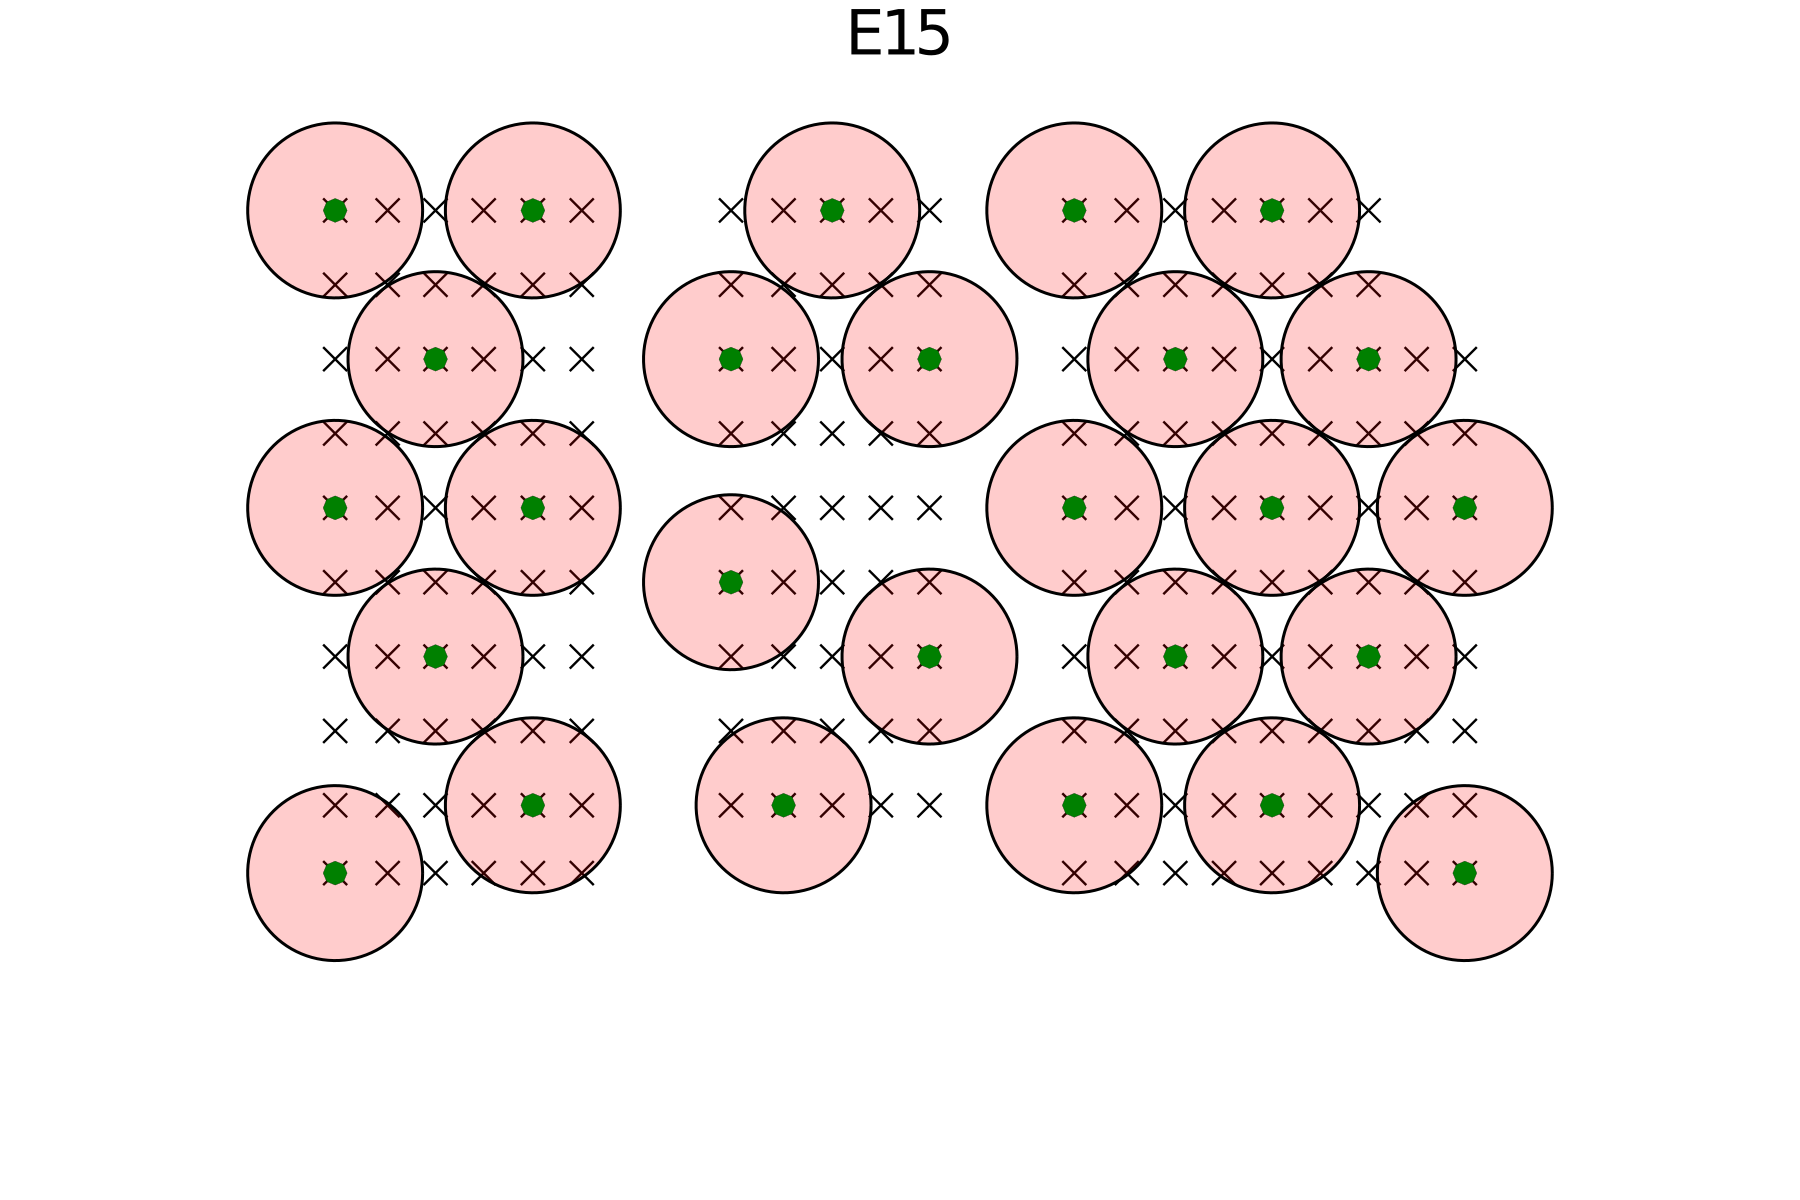
\includegraphics[width=0.93\textwidth]{E15_26_circles.png}
         \label{fig:E15}
     \end{subfigure}        
     \hfill
     \vspace{-2cm}
     \begin{subfigure}[b]{1\textwidth}
         \centering
         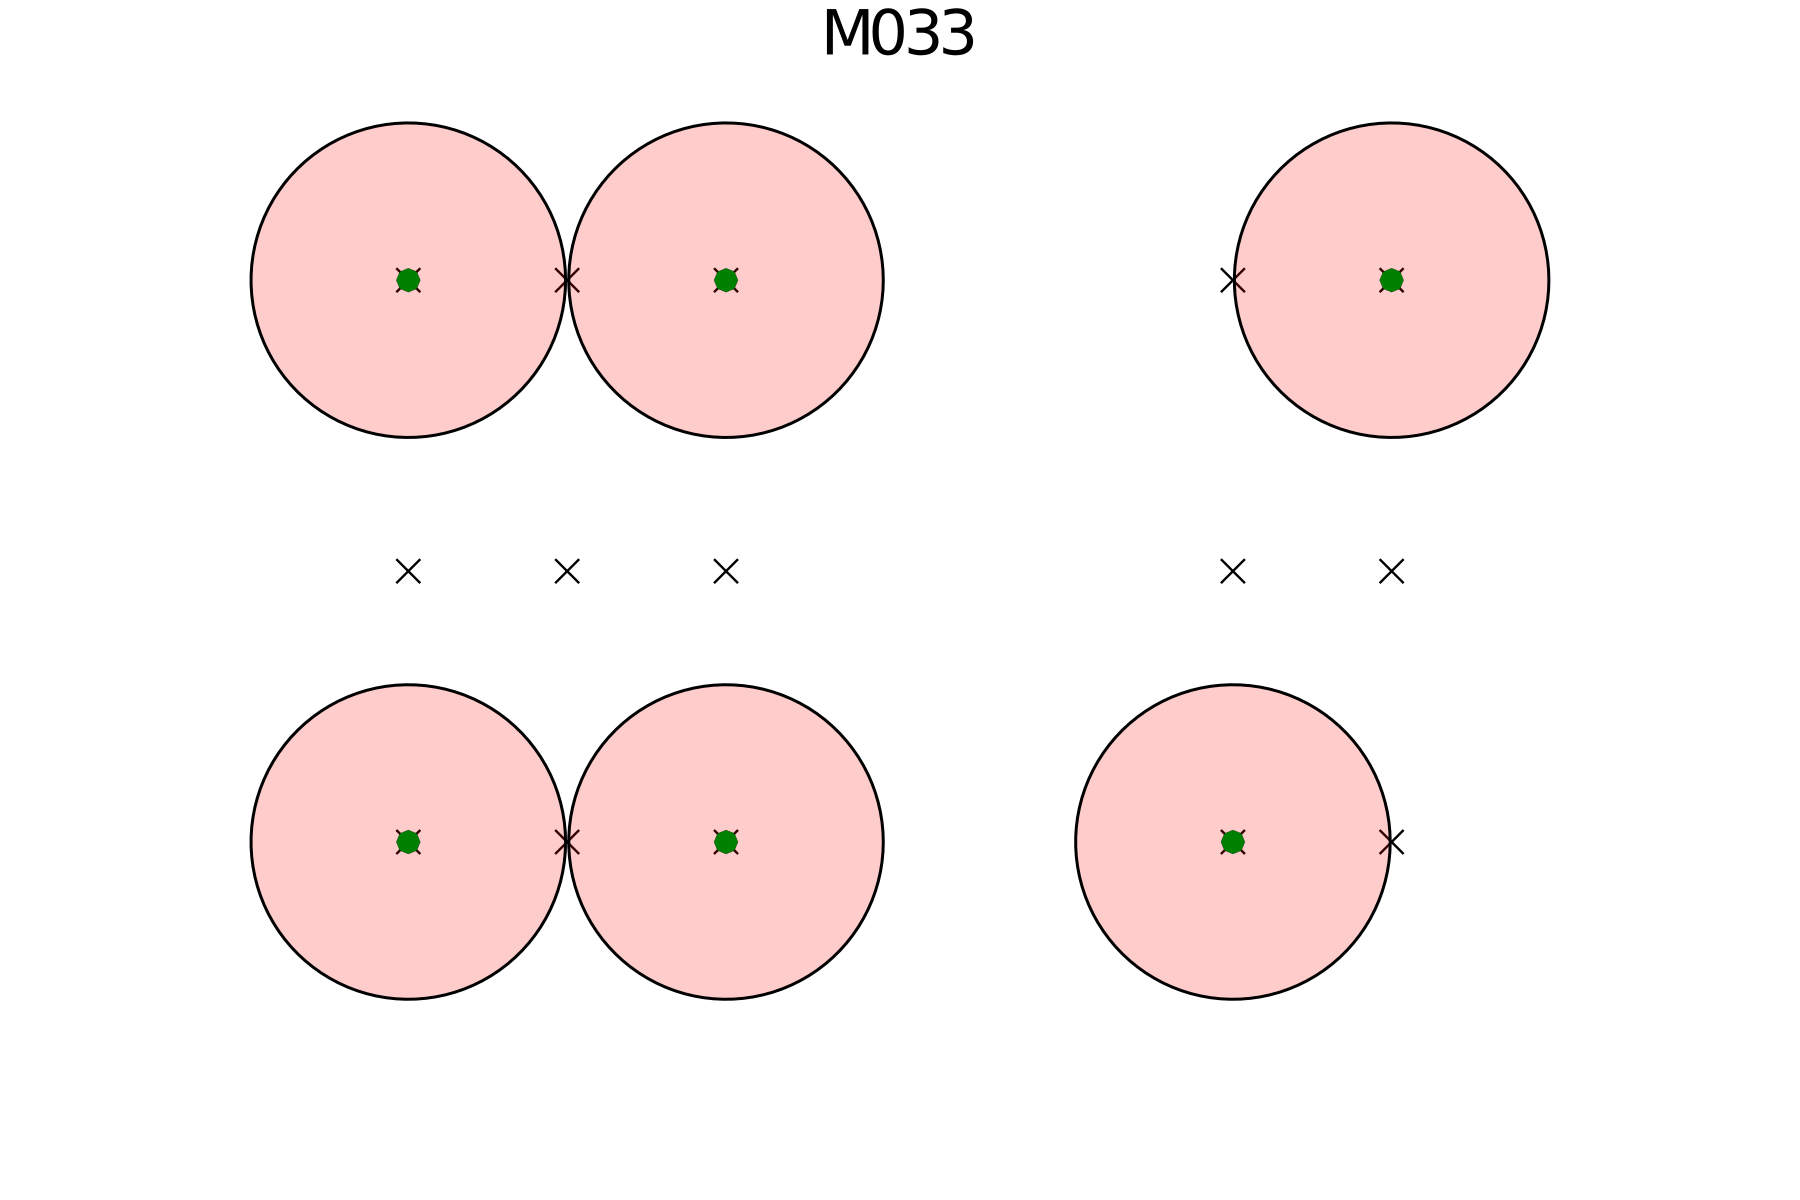
\includegraphics[width=0.93\textwidth]{M033_6_circles.png}
         \label{fig:M033}
     \end{subfigure}
         \hfill
         \caption{Optimised seating layouts for E15 and M033 using a social distancing measure of 2 metres. The crosses mark the locations of available seats, green markers are the locations of socially distanced seats, which are enclosed by a circle of radius 1m to highlight no overlap between socially distant seats.}
        \label{fig:E15 and M033}
\end{figure}

\begin{figure}[H]
         \centering
 \begin{subfigure}[b]{1\textwidth}
         \centering
         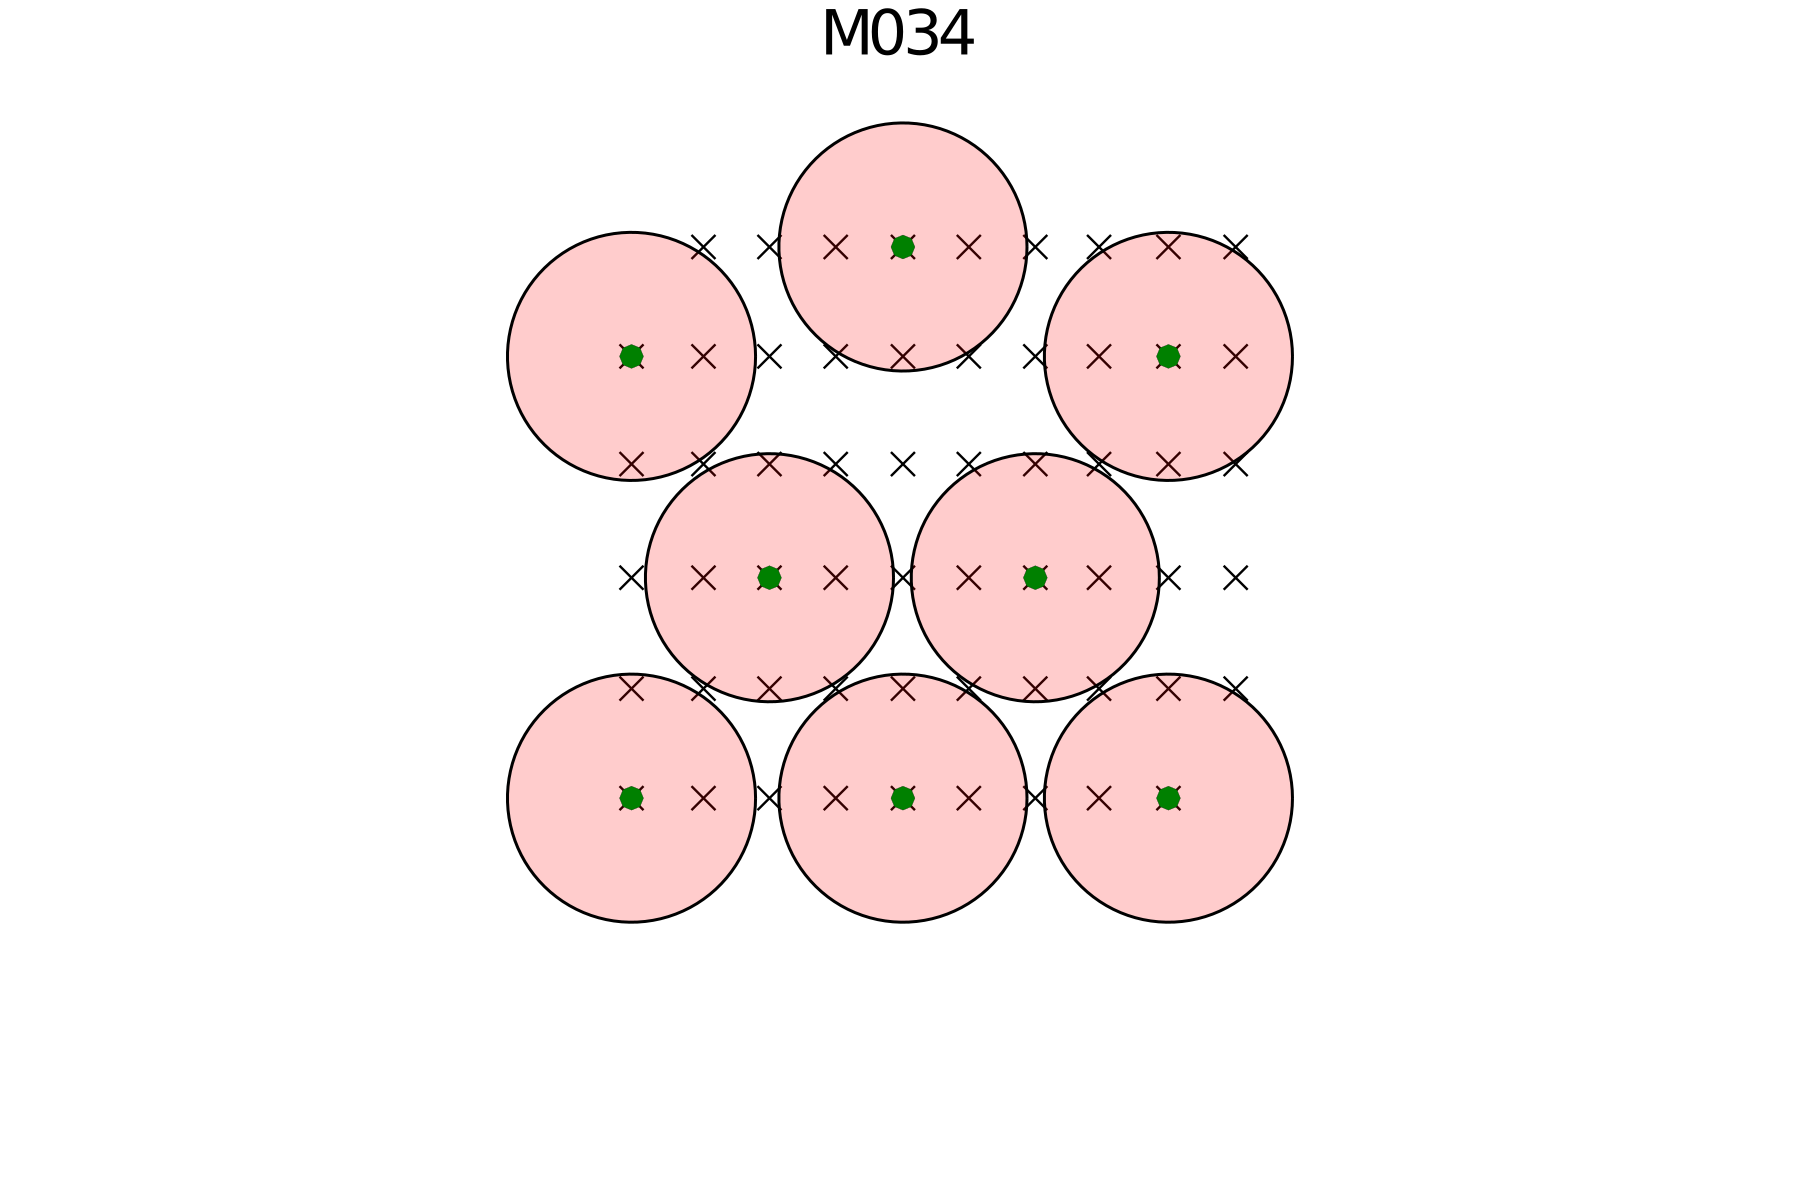
\includegraphics[width=0.97\textwidth]{M034_8_circles.png}
         \label{fig:E15}
     \end{subfigure}        
     \hfill
     \vspace{-2cm}
     \begin{subfigure}[b]{1\textwidth}
         \centering
         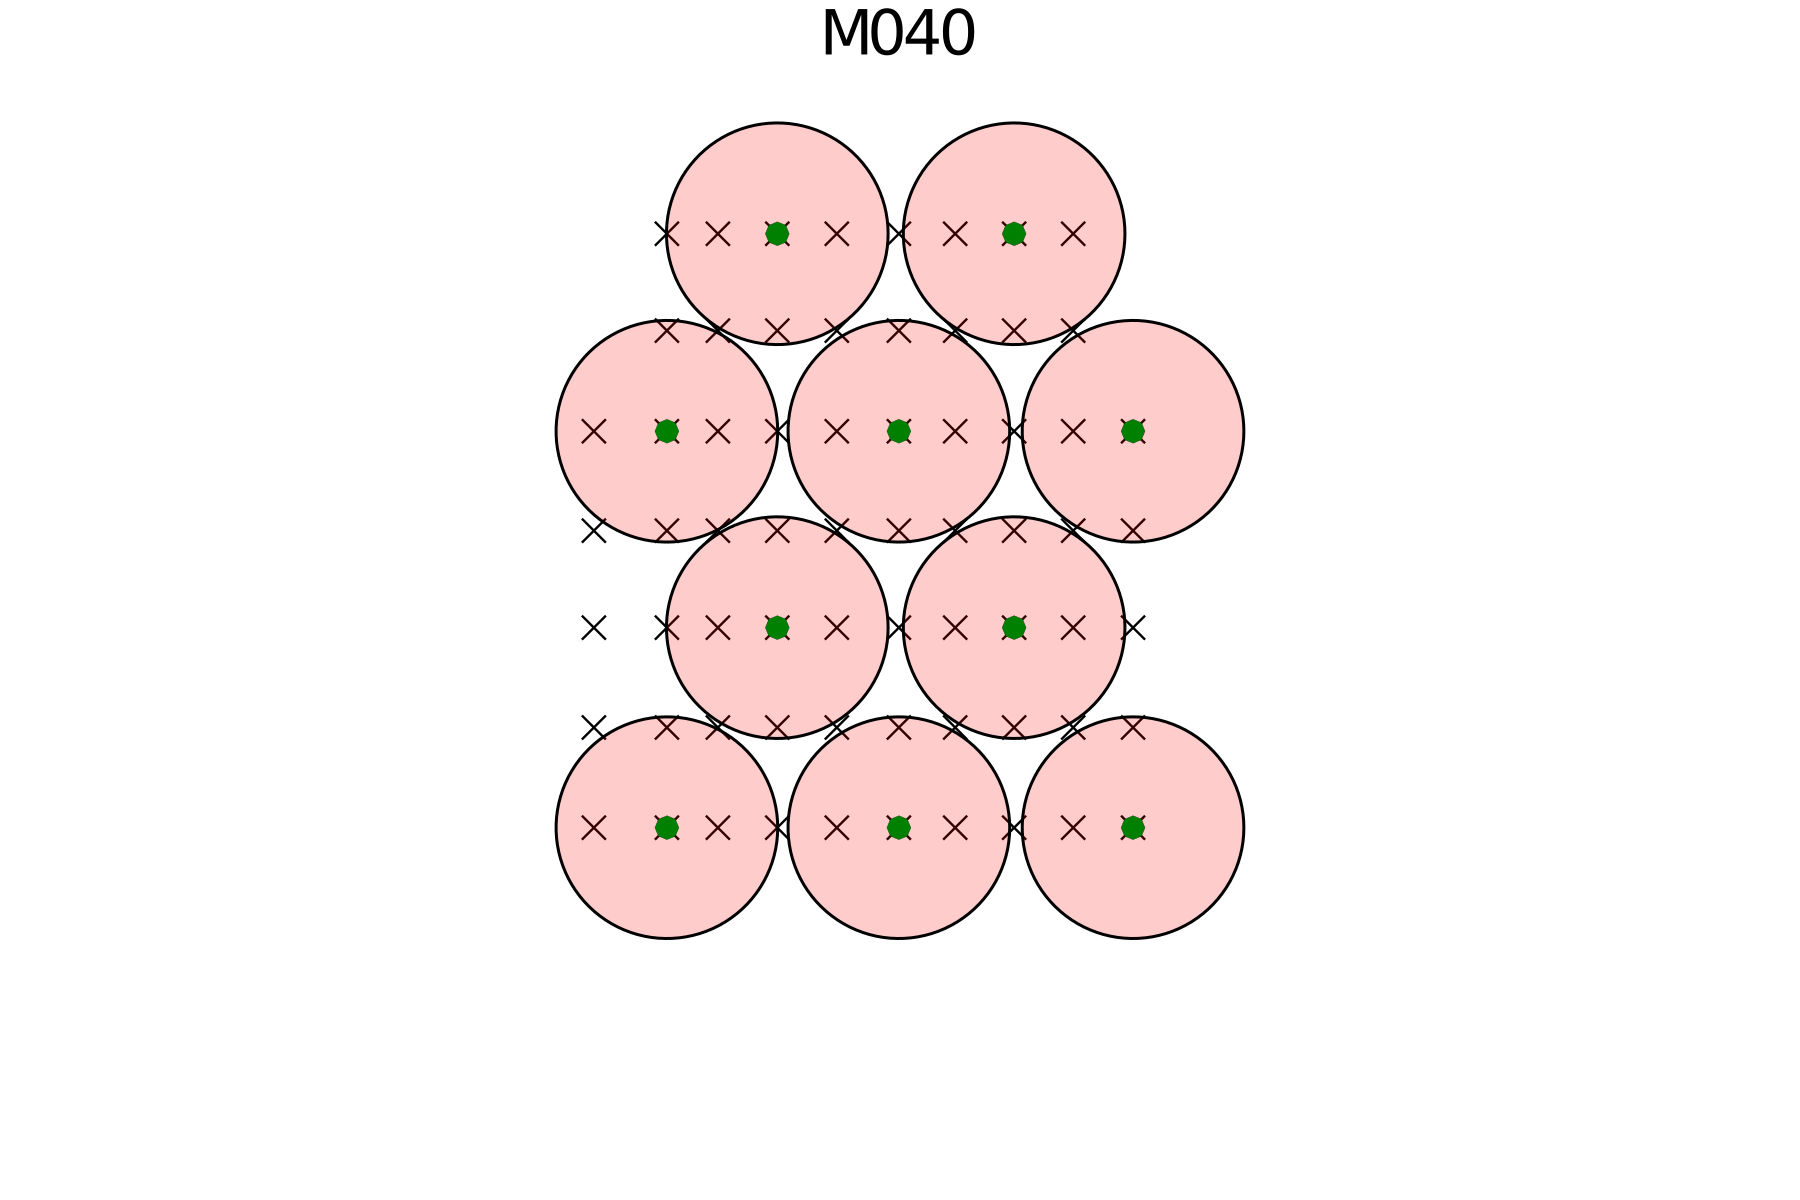
\includegraphics[width=0.97\textwidth]{M040_10_circles.png}
         \label{fig:M033}
     \end{subfigure}
         \hfill
         \caption{Optimised seating layouts for M034 and M040 using a social distancing measure of 2 metres. The crosses mark the locations of available seats, green markers are the locations of socially distanced seats, which are enclosed by a circle of radius 1m to highlight no overlap between socially distant seats.}
        \label{fig:M034 and M040}
\end{figure}


\section*{Disclaimer}
Any information provided is based on a purely mathematical argument and so there may exist external factors that have not been considered, therefore, the provided information should be used only as guidance. \textbf{The welfare of those occupying the space should always be the highest priority}. The accuracy of our solutions is dependent on the quality of the data supplied, please take all necessary steps to validate supplied data and received information with the physical spaces considered. We are not responsible of the decision of appropriate social distancing measure, this responsibility lies with the client and should always be in agreement with UK government guidelines. \textbf{Any action taken upon receiving information from our team is strictly at your own risk}. We make no representation that our services will provide any enhancement to current operational targets. 

\end{document}